Для каждого изображения вклад микролинзирования уникален и не зависит от других изображений, что вносит некоторую неопределенность в определение временных задержек между изображениями. Для количественных оценок точности определения $\Delta t$ между двумя кривыми блеска с учетом микролинзирования используется подход, детально описанный в работе \cite{doblerkeeton2006} -- пионерской работе по этому направлению. За основу была взята одна из кривых блеска SN Refsdal, рассчитанных в гидродинамической модели в различных частотных фильтрах для 400 дней с момента её взрыва (Бакланов и др., в подготовке). Она изображена на Рисунке \ref{fig:lightcurves}. 

\begin{figure}[H]
    \centering
	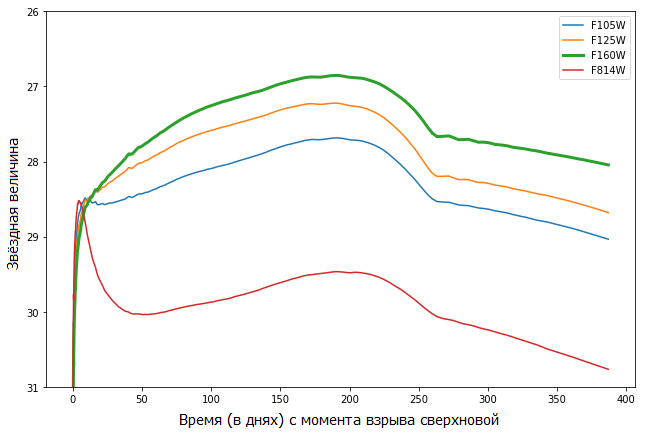
\includegraphics[scale=0.68]{pics/lightcurves.png}
	\caption{Кривые блеска SN Refsdal в различных фильтрах, полученные в гидродинамической модели (Бакланов и др., в подготовке). \label{fig:lightcurves}} 
\end{figure}

Для простоты анализа рассматривается кривая блеска только в одном фильтре - F160W. Для иллюстрации влияния микролинзирования используются карты для областей изображений S1 и S2 (см. Рис. \ref{fig:s1s4}). SN Refsdal моделируется кругом с постоянной поверхностной яркостью, случайно расположенным на карте, расширяющимся со скоростью 5000 км/с. Выбор такого значения скорости в некоторой степени произволен (для иллюстрации), но по порядку величины соответствует действительному, оцениваемому как $v \sim {R_{SN}^{max}}/{t_{\textrm{расширения}}} \sim {2 \cdot 10^{15} \textrm{см} }/{55 \textrm{ суток}}$.

Предполагается, что оригинальная кривая блеска наблюдается в изображении S1. Для имитации изображения S2 имеющаяся кривая блеска дублируется и сдвигается по времени (далее эта разница обозначается как истинная временная задержка $\Delta t_{\textrm{ист.}}$) и звёздной величине относительно оригинальной. После этого к каждой из кривых блеска добавляются уникальные “шумы”, вызванные микролинзированием, полученные при помощи программного пакета {\tt{SNTD}} на соответствующих картах. Для “зашумленных” кривых блеска временная задержка между изображениями определяется путем минимизации следующего функционала (аналогично работе \cite{doblerkeeton2006}:

\begin{equation}\label{chi2}
\chi^{2}(\Delta t)=\frac{1}{N} \sum_{i=1}^{N} \frac{1}{\sigma_{i}^{2}}\left[D^{+}\left(t_{i}\right)-D^{-}\left(t_{i}-\Delta t\right)-k\right]^{2}
\end{equation}
где $D^+$ и $D^-$ - значения кривых блеска, выраженные в звёздных величинах, $\sigma_i$ - фотометрическая погрешность с нормальным распределением (она предполагается постоянной во времени), $k$ - нормировочная постоянная, связанная с различным макроусилением псевдо-изображений. Далее эта операция многократно повторяется, после чего по полученным значениям разброса временных задержек находится стандарное отклонение соответствующего распределения $\Delta t$ по формуле
\begin{equation}\label{sigmadeltat}
\sigma_{\Delta t}=\sqrt{\frac{1}{N} \sum_{i=1}^{N}\left((\Delta t)_{i}-\overline{\Delta t}\right)^{2}},
\end{equation}
которую можно трактовать как показатель неопределённости, вызванной микролинзированием, во временной задержке между изображениями. Результаты представлены в следующей секции.
